In this section, we introduce the cross-validation estimation for LS-SVM. As we mentioned in Section \ref{sec:single:comb} that once we determine the value of the transfer parameters $\gamma$, problem \eqref{eq:single:unionreg} can be solved directly. In Section \ref{sec:single:comb}, we treat the transfer parameters as the parameters to be set in advance. In this section, we introduce how we can estimate the unbiased transfer parameters by using an important property of LS-SVM for parameter estimation. 

\subsection{Closed Form Cross-validation Estimation for LS-SVM}
To estimate the transfer parameter, we adopt cross-validation for parameter estimation. Cross-validation is widely used for parameter estimation. Suppose we have a model with one or more unknown parameters, and a data set to which the model can be fit (the dataset). The fitting process optimizes the model parameters to make the model fit the data as well as possible. On the other hand, we have to make sure that this model have the generalization ability, i.e. it can also work well on other independent validation dataset. Otherwise, the model is overfitted to the training data set. However, in practical problem we may not be able to get another independent data set except for the original dataset. Therefore, we have to manually create the validation set by selecting some of the data from the original dataset and use them for evaluation. One round of cross-validation involves partitioning a sample of data into complementary subsets, performing the analysis on one subset (called the training set), and validating the analysis on the other subset (called the validation set or testing set). By repeating these process several rounds with different partitions, we can significant reduce the variability of our estimation using the average results over the rounds.
\begin{figure}
	\centering
	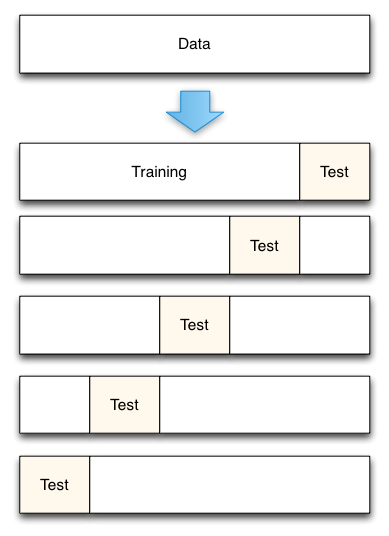
\includegraphics[scale=.4]{transfer/fig/cv.png}
	\caption{An illustration of 5-fold cross-validation}
\end{figure}
There are several different types of cross-validation methods due to their partition strategies. K-fold cross-validation is the most popular type among them. In k-fold cross-validation, the original dataset is randomly partitioned into k equal sized subsamples. K-fold cross-validation is performed in K rounds and in each round, each one of the K partition is used exactly once as the validation set and the rest partitions are used as the training set. 

In our work, we also employ cross-validation for parameter estimation. Here we show that the cross-validation error for LS-SVM can be represented in an efficient way. As a result, we don't have to actually perform cross-validation and re-train the models in each round to obtain the cross-validation error.

\begin{theorem}[An extension of \cite{cawley2006leave}]\label{th:single:cv}
	Given a dataset $D=\{(x_i,y_i)|i=1,...,l\}$, the solution of a LS-SVM on $D$ can be written as Eq. \eqref{eq:gama:lssvm}.
	Assume that $D^{(n)} = \{(x_i,y_i)|i=1,...,n\}$ is a subset of $D$ and $D\backslash D^{(n)}$ is the complement of $D^{(n)}$ in $D$. 
	Let $\left[\alpha_1,...,\alpha_n\right]$ be the corresponding $n$ rows of $\alpha$ in Eq. \eqref{eq:single:orgmatrix} and $S_n$, $s$ and $S_{(l - n + 1)}$ represent the square blocks of matrix:
	
	\begin{equation*}
	\left[ {\begin{array}{c|c}
		{{S_{n }}} &s\\ \hline
		{{s^T}}&{{S_{(l - n + 1)}}}
		\end{array}} \right] =\left[ {\begin{array}{*{20}{c}}
		{K  + \frac{1}{C}{\rm I}}\\
		1^T
		\end{array}\begin{array}{*{20}{c}}
		1\\
		0
		\end{array}} \right]
	\end{equation*}
	The unbiased leave out error of a LS-SVM trained from $D\backslash D^{(n)}$ on $D^{(n)}$ can be estimated as:
	
	\begin{equation*}\label{eq:single:nout}
	ERR_{leave-out} = \left( {{S_n} - sS_{(l - n + 1)}^{ - 1}{s^T}} \right){\left[ {{\alpha _1},...,{\alpha _n}} \right]^T}
	\end{equation*}
\end{theorem}
We show the proof in Appendix \ref{app:cross}. This remarkable result allows cross-validation to be used while only fitting the model once to all available data.

Therefore, we have a convenient solution to estimate the unbiased cross-validation error. However, to perform a cross-validation in practice, decide the partition strategy. Suppose we have $l$ examples in the original data and we want to perform a K-fold cross-validation on it. Thus we have $\mathbf{C^{l/K}_l}$ possible combinations. This means larger K leads to less computation time. Moreover, larger K means less bias towards overestimating the true expected error (as training folds will be closer to the total dataset). When we set $K=l$, we perform $l$-fold cross-validation, i.e. leave-one-out cross-validation (LOO-CV). Vapnik et al. \cite{vapnik2000bounds} show that LOO-CV can provide an almost unbiased estimation error. Previous work also show that transfer learning on the small target training set can be benefit from LOO-CV to better estimate the transfer parameters as well as prevent negative transfer \cite{kuzborskij2013stability}. Due to the reasons above, in this thesis, we use LOO-CV to estimate the transfer parameters to optimize our transfer model.

According to Theorem \ref{th:single:cv}, the LOO-CV error for LS-SVM can be represent as:
\begin{equation}
	ERR_{loo}=\frac{1}{l}\sum_{i}^{l}
\end{equation}